\chapter{Realidade Virtual - Áreas de aplicação}

Após uma apresentação do conceito e da história da \acl{RV}, este capítulo vem apresentar um conjunto de aplicações ligadas atualmente à \acl{RV}\footnote{Apenas alguns exemplos de áreas de aplicação.}.
 
\section{Medicina}

\subsection{Treino Médico}
Esta área de aplicação permite que os pacientes tenham uma melhor interação e compreensão sobre o corpo humano, construindo e/ou reaprendendo novas capacidades que serão posteriormente aplicadas em situações reais. Todas estas novas habilidades são realizadas em ambiente virtual, garantindo assim a máxima segurança dos pacientes.
Em ambiente de ensino, podemos dar o exemplo da Odontologia, onde os alunos podem trabalhar por um conjunto de dentes em \emph{3D} e executar uma série procedimentos clínicos próprios, como por exemplo, uma broca virtual.

\subsection{Paramédicos}
Na área dos Paramédicos e outras atividades equivalentes, a \acl{RV} é também utilizada em treinos de medicina. Com isto, os futuros médicos aprendem a desenvolver novas capacidades de socorro rápido sem colocar ninguém em risco. 

\subsection{Tratamento de Fobias}	
No tratamento de fobias a \acl{RV} também tem a sua aplicação. Por exemplo, tratar pacientes que tenham medo de andar de avião, de estar em alturas ou estar na presença de determinados animais. O paciente sabe que está num ambiente totalmente seguro, mas o cérebro confunde-se e reage como se da realidade se tratasse. Com isto torna-se muito mais simples para o médico ajudar o paciente e também poderá aumentar ou diminuir a dificuldade do tratamento.

\begin{figure}[h]
\center
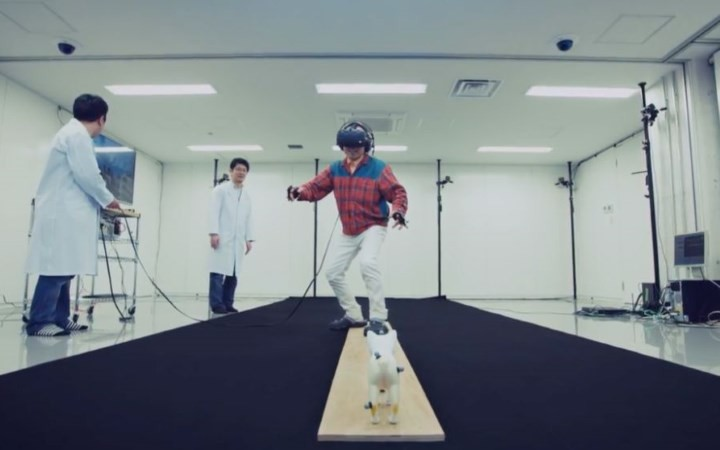
\includegraphics[scale=0.4]{imagens/RV_tratamento_fobia.jpg}
\caption{Exemplo do tratamento da fobia de alturas. Simulação em RV \cite{RV_fobia_1}}
\end{figure}

\section{Jogos}
Na década de 80 e 90 várias foram as empresas que tiveram a tentativa de começar com a \acl{RV} mas sem sucesso, isto porque não haviam recursos computacionais suficientes para que tal fosse possível. As empresas estavam mais focadas em tentar relacionar a Realidade Virtual com jogos, temos o exemplo, já mencionado noutro capitulo, da SEGA que em 1993 anunciou os \emph{Sega VR headsets}, mas devido a problemas a empresa desistiu do produto, nunca tendo chegado ao mercado.

Em 2009 a \emph{Palmer Luckey}, na garagem dos seus pais criou o primeiro protótipo do \emph{Oculus Rift}. Foi este o inicio dos óculos virtuais \cite{RV_fundador}.

Mais tarde, a playstation lançou a \emph{Playstation VR}. A \emph{Playstation VR} utiliza o comando da \emph{PS4} e um comando semelhante ao da \emph{Nintendo Wii}, que reconhece os movimentos do usuário e assim a experiência torna-se muito mais real.

A \emph{HTC} também juntou-se a este mercado em parceria com a \emph{Valve} anunciando o \emph{HTC Vive}.
este equipamento exige que o utilizador adquira um computador potente e que tenha mais espaço disponível. Até agora o \emph{HTV Vive} é o único que tem comandos especialmente desenvolvidos para uma maior interação.


\section{Simuladores}
\subsection{Simulador de Comboio}

Os Simuladores de Comboios permitem emular exatamente o comportamento do comboio, tendo como objetivo ser uma ferramenta prática e confiável para o treino dos maquinistas.

Existem diversos elementos que constituem este sistema, desde a escolha da locomotiva, travões, potência, modelo etc. O sistema é capaz de simular a condução normal de um comboio e para além disso também é capaz de reproduzir várias condições atmosféricas. O sistema também permite a configuração do comboio, simulando degradações no mesmo de forma a avaliar a capacidade do maquinista \cite{RV_comboio}.


\subsection{Simulador de Voo}

Do mesmo modo que os simuladores de comboios, os simuladores de voo são utilizados para o treino de pilotos. Estes têm como objetivo atribuir qualificações aos tripulantes técnicos. Somente nestes equipamentos é possível treinar e simular diversas situações com grande realismo, isto sem por em risco a vida das pessoas.
O uso deste tipo de simuladores de voo no âmbito de treinar, proporciona uma enorme economia em combustível. Como consequência, o custo das formações será mais reduzido assim como o impacto no ambiente, porque não haverá queima de combustível, reduzindo assim os gases carbónicos que são emitidos \cite{RV_aviao}.

\begin{figure}[h]
\center
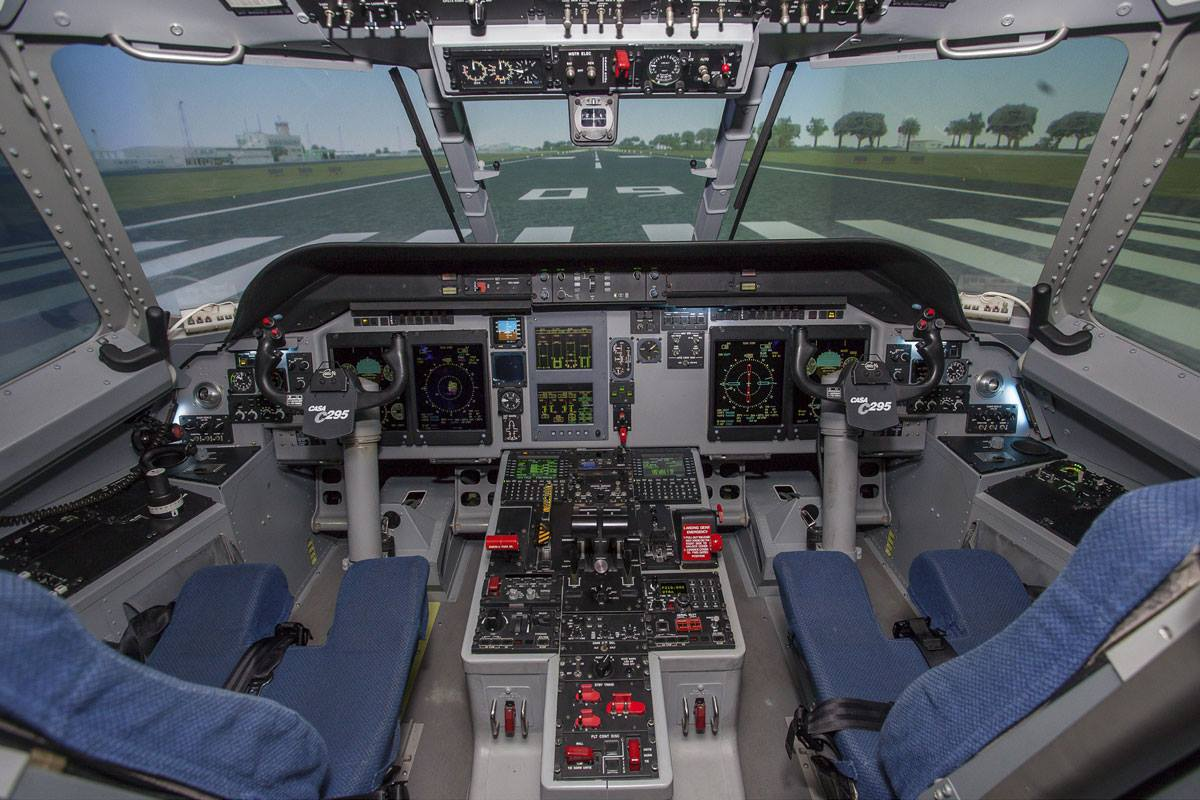
\includegraphics[scale=0.2]{imagens/RV_simulador_voo.jpg}
\caption{Exemplo de um simulador de voo. \cite{RV_sim_voo}}
\end{figure}

\section{Área militar}

Na industria militar também a realidade virtual é aplicada em simuladores, sendo o seu principal objetivo treinar militares num ambiente seguro sem qualquer tipo de consequências. 

A Força Aérea, o Exército e a Marinha usam por exemplo, os simuladores de voo, no âmbito de treinar os seus pilotos. Alguns exemplos desta simulação é abastecer em caso de emergência ou voar num campo de batalha ou até mesmo como coordenar a sustentação no ar com ajudar de operações terrestres \cite{RV_militar}.





